\documentclass[tikz, crop, border = {2pt 2pt 2pt 2pt}]{standalone}

\usepackage{concmath-otf}
\usepackage{esvect}

\usetikzlibrary{calc}

\begin{document}
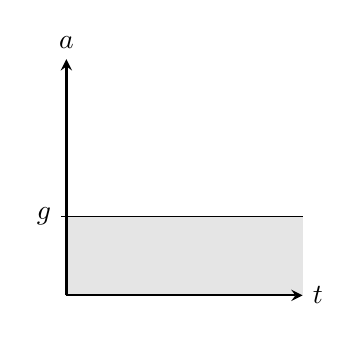
\begin{tikzpicture}
    \draw[-stealth, thick] (0, 0) -- (3, 0) node[right]{$t$};
    \draw[-stealth, thick] (0, 0) -- (0, 3) node[above]{$a$};

    \fill[color = lightgray!40, blend mode = multiply] (0, 0) rectangle (3, 1);
    \draw (0, 1) -- ++ (3, 0);

    \draw (2pt, 1) -- ++ (-4pt, 0) node[left]{$g$};
\end{tikzpicture}
\end{document}